\chapter{بررسی نحوهٔ فشرده‌سازی در فرمت MP3}
\noindent
\textbf{
	\textit{
        توضیح نحوهٔ کار فشرده‌سازی در فرمت \lr{MP3}،
        تحلیل صدای انسان و توضیح کانال‌های فرکانسی
	}
}
\pagebreak

\section{ مقدمه}
در اواخر قرن بیستم و با شروع فراگیری اینترنت در جوامع مختلف، اشتراک‌گذاری 
مدیا‌های مختلف مانند صوت، فیلم و تصویر در فضای اینترنت به یکی از خواست‌های همگانی و نیازهای اصلی مردم تبدیل شد اما 
مشکل اصلی در این میان، حجم زیاد فایل‌های مدیا و سرعت پایین انتقال داده در فضای اینترنت بود، 
فرمت‌های فشرده‌سازی مختلفی برای حل این معضل پیشنهاد شدند که هر کدام با تکیه بر
تحلیل‌های آماری و یا حذف داده‌هایی غیرضروری در راستای کم کردن حجم فایل‌های مدیا می‌کوشیدند. در زمینهٔ  فشرده‌سازی فایل‌های
صوتی فرمت MP3 یقینا فراگیرترین و موفق‌ترین فرمت به شمار می‌رود. در این فصل 
نگاهی کلی به نحوهٔ کار این فرمت و الگوریتم‌های با هدررفت داده به کاررفته در این فرمت خواهیم داشت. برای تقریب اذهان به بزرگی حجم فایل‌های صوتی فشرده‌ناشده لازم به توجه است که هر
فایل صوتی در حالتی که هیچ مقداری از داده فشرده نشود در هرثانیه حدود ۱۷۶۰۰۰ بایت فضا می‌گیرد.

\section{نرخ بیتی } 
برای درک بهتر مفاهیمی که در ادامهٔ متن با آن‌ها سر و کار داریم لازم است تا ابتدا با مفهوم نرخ بیتی \footnote{bitrate} آشنا شویم، در مفاهیم علوم کامپیوتر، نرخ بیتی
معمولا  مقدار بیتی‌ست که در برای واحد زمانی ذخیره می‌شود، مثلا وقتی bitrate یک موسیقی 
\lr{320 kb/s }
اعلام می‌شود به این معنی‌ست که برای هر ثانیه از این صوت ۳۲۰ کیلوبیت داده ذخیره شده است؛ همچنین نرخ بیتی می‌تواند سرعت انتقال داده در یک
کانال را بیان کند،‌ مثلا در طراحی مودم‌های شبکه از این مفهوم برای نمایش سرعت انتقال داده استفاده می‌شود. 

\section{نحوهٔ کار mp3}
تمرکز فرمت mp3 در فشرده‌سازی 
بر حذف اصواتی‌ست که توسط گوش انسان شنیده نمی‌شوند،‌ همان‌طور که از فصل دو به یاد دارید برای فشرده‌سازی تصاویر می‌توانستیم از بیت‌هایی که 
نمایان‌گر تصاویری با فرکانس بالا بودند صرف نظر کنیم زیرا توسط چشم انسان قابل تشخیص نبودند،‌ در فشرده‌سازی صوت نیز می‌توانیم 
 با مطالعهٔ ساختار شنوایی انسان اصواتی که به طور معمول توسط گوش انسان شنیده نمی‌شنود را از صوت حذف می‌کنیم تا حجم فایل کاهش یابد.

 به شکل خلاصه می‌توان مراحل فشرده‌سازی در فرمت mp3 
 را به شکل زیر خلاصه کرد.

 \begin{itemize}
         \item تبدیل صوت به قسمت‌های کوچک
         \item حذف صوت‌های خارج از محدودهٔ شنوایی انسان
         \item نمونه‌برداری از موسیقی با توجه به نرخ بیتی خواسته شده
         \item اضافه کردن افزونه‌ها و فشرده‌سازی نمونه
 \end{itemize}

\section{بررسی دستگاه شنوایی انسان}
برای فشرده‌سازی صوت باید در ابتدا اصواتی که توسط گوش انسان قابل شنیدن نیستند یا گوش انسان با جزییات کمتری آن‌ها را درک می‌کند را حذف کنیم، برای 
این کار به تحلیل صوت‌شناسی
\footnote{Psychoacoustics}
نیاز دارد. 

نتایج تحلیل‌های صوت‌شناسی برای دستگاه شنوایی انسان موارد مفید زیر را اعلام می‌کند. 

\begin{itemize}
        \item ضعف شنوایی بزرگسالان
        \item درک کمتر جزییات صداهای کم
        \item آستانهٔ شنوایی انسان
        \item اثر پوشش‌دهی صداهای بلند
\end{itemize}

به تفصیل موارد بالا و کاربرد‌های آنان در فشرده‌سازی را بررسی خواهیم کرد.

\subsection{ضعف شنوایی بزرگسالان}
در کودکی انسان‌ها معمولا می‌توانند اصواتی را که بین فرکانس‌های 0.1 تا ۲۰ کیلوهرتز باشند را بشنوند، اما با بزرگ شدن انسان معمولا حد بالای شنوایی 
به مقدار ۱۵ کیلوهرتز می‌رسد و در صورتی که به درصد فشرده‌سازی بالایی نیاز داشته باشیم می‌توانیم از فرکانس‌های بیش از ۱۵ کیلوهرتز صرف نظر کنیم.

\subsection{درک کمتر جزییات صداهای کم}
دستگاه شنوایی انسان معمولا به جزییات صداهای بلند بیش از صداهای آرام توجه می‌کند، در نتیجه می‌توانیم برای صداهایی که 
سطح فشار صوت \footnote{\lr{Sound Pressure Level (db)}}
 کمتری دارند از bitrate پایین‌تری استفاده کنیم. 

 \subsection{آستانهٔ شنوایی انسان}
 گوش انسان برای هر فرکانس صوتی آستانهٔ شنوایی دارد که اگر سطح فشار صدا از آن کمتر باشد آن را نمی‌شنود، 
 شکل 
 \ref{human_hearing}
 این آستانه را برای فرکانس‌های مختلف نشان می‌دهد؛ در صورتی که سطح صوتی فرکانسی در هر قسمت از مقدار آستانهٔ آن کمتر باشد آن صدا شنیده نمی‌شود و 
 می‌توان آن را حذف کرد.

 \begin{figure}[]
         \centering
         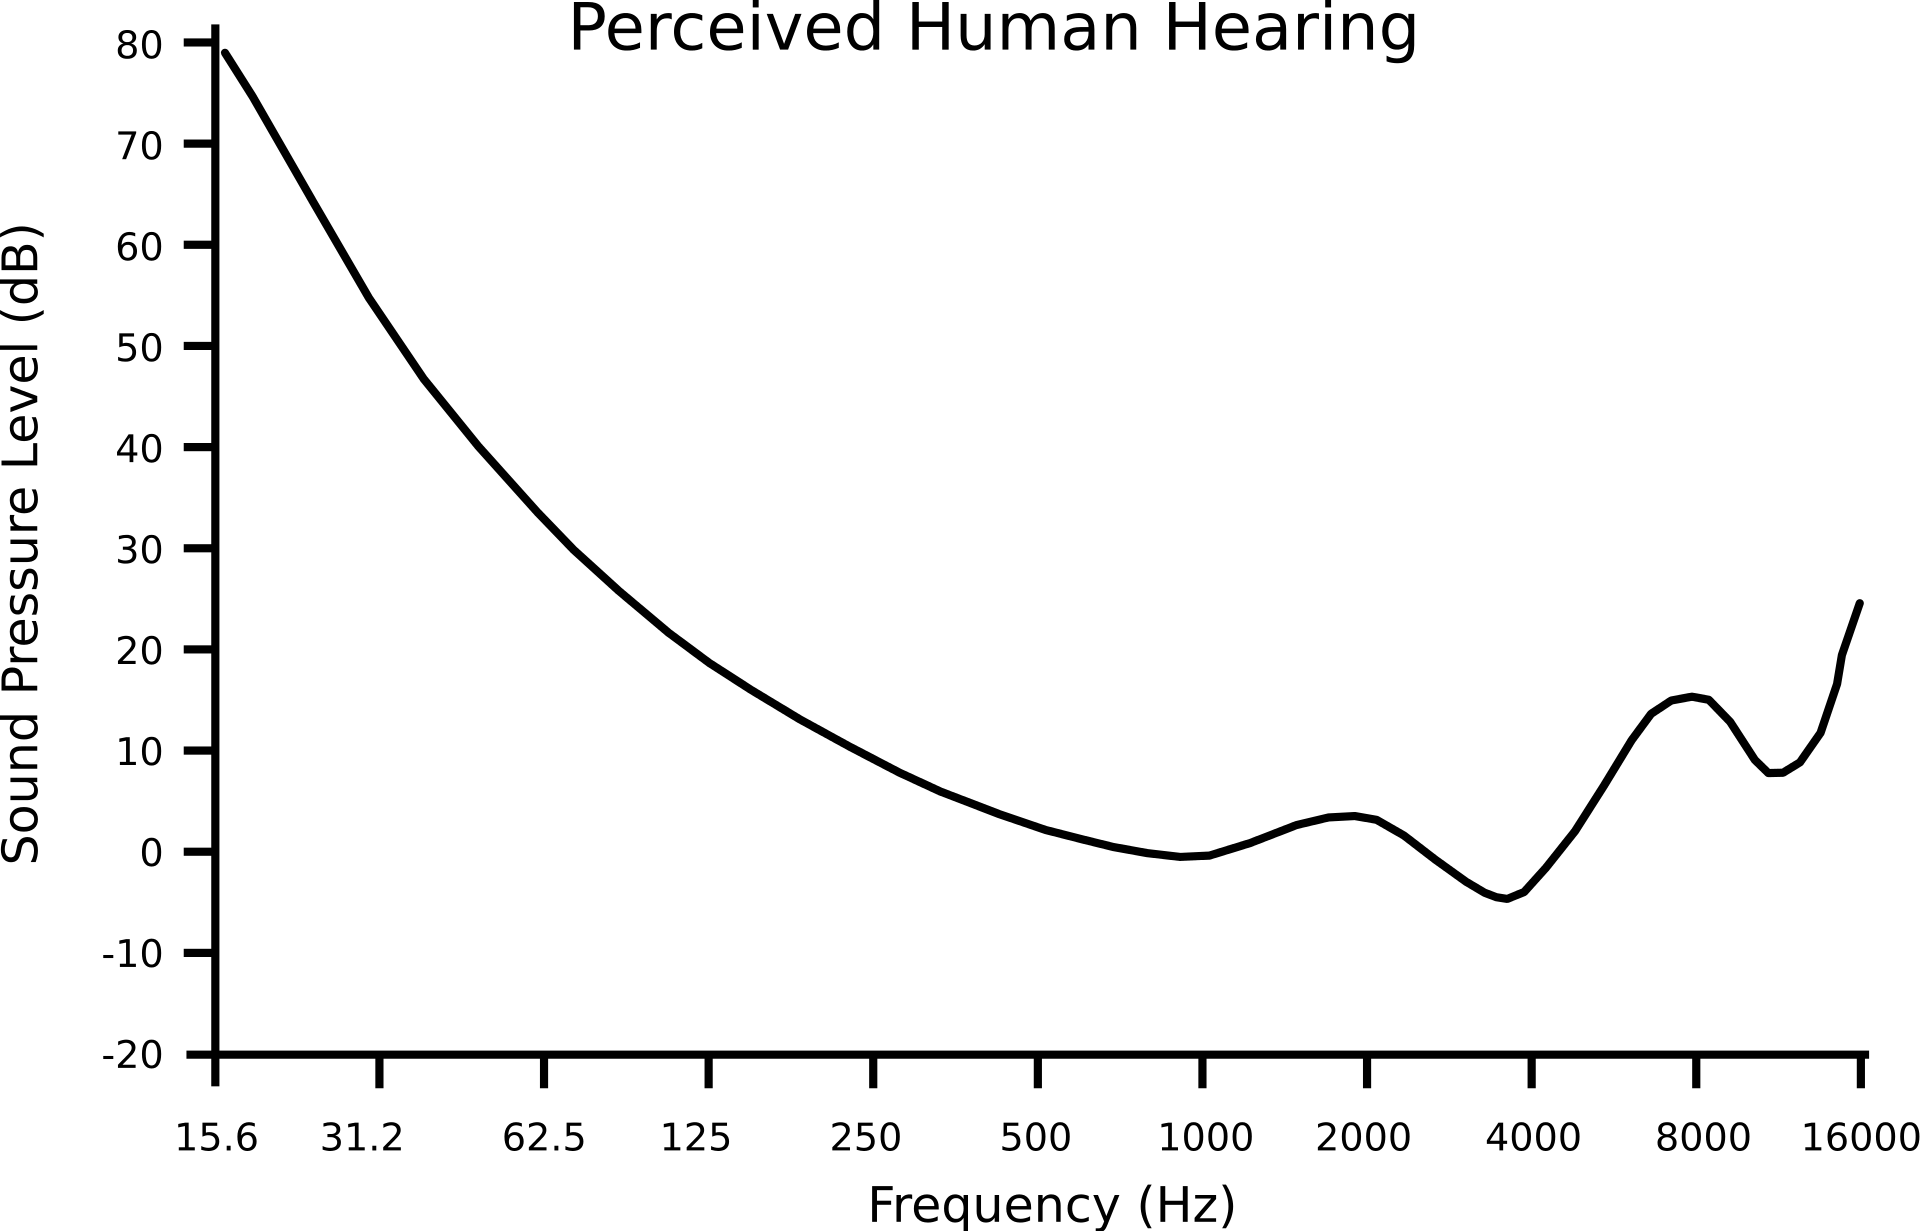
\includegraphics[width=\textwidth]{figs/human_hearing.png}
         \caption{آستانهٔ شنوایی انسان برای فرکانس‌های مختلف}
         \label{human_hearing}
 \end{figure}
 \subsection{اثر پوشش‌دهی صداهای بلند}
 هنگامی که در یک محدودهٔ فرکانسی یک صدای بلند رخ دهد گوش انسان نمی‌تواند صداهای آرام با فرکانس‌های نزدیک به آن را تشخیص دهد و بشنود
 حتی اگر سطح صوتی آن از آستانهٔ شنوایی انسان بیشتر باشد، به این اثر در گوش انسان اثر پوشش‌دهی 
 \footnote{\lr{Masking Effect}} 
 گفته می‌شود. 
 مثالی از اثر پوشش‌دهی در شکل 
 \ref{masking_effect}
 نشان داده شده است. 

 \begin{figure}[]
         \centering
         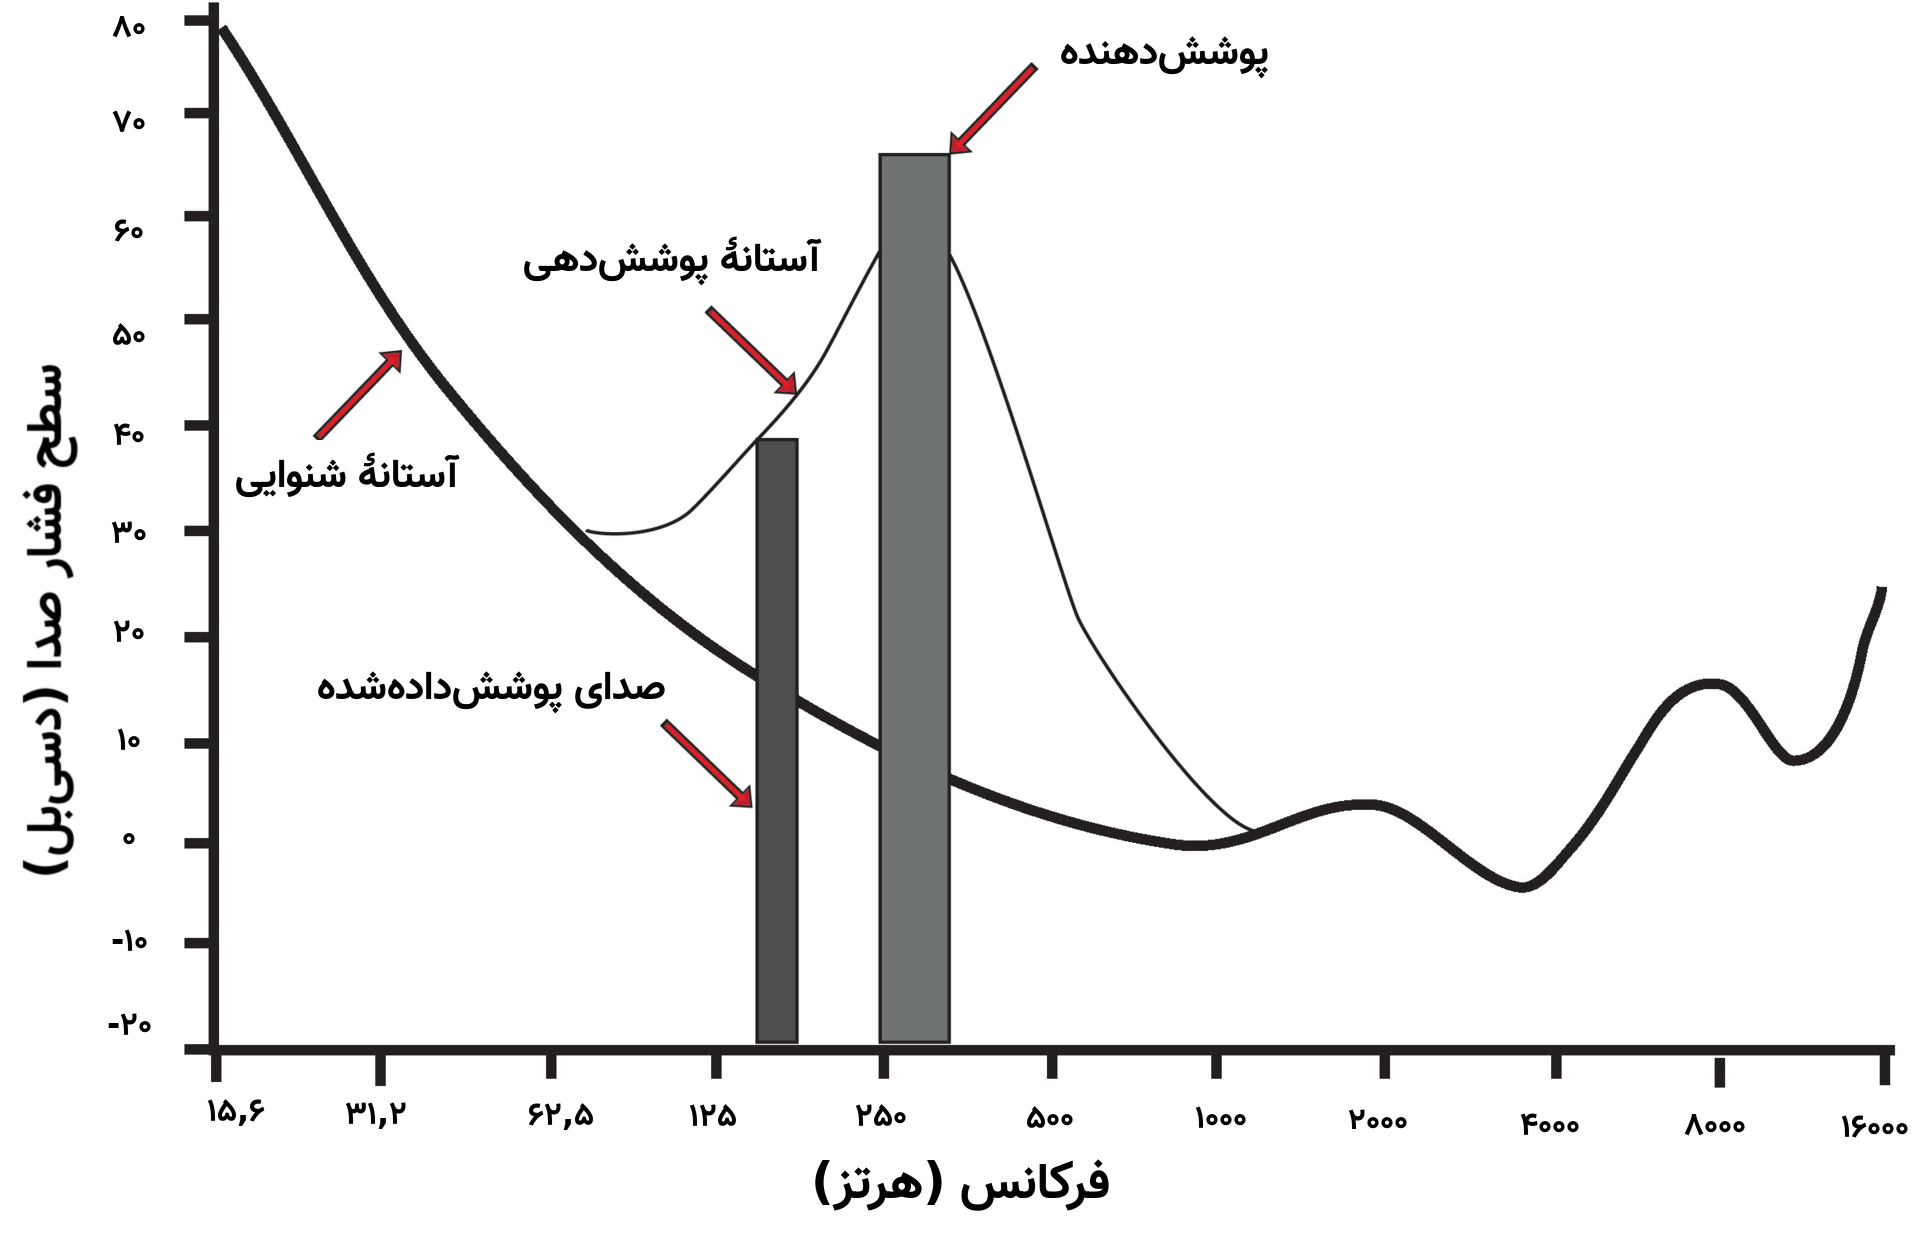
\includegraphics[width=\textwidth]{figs/masking_effect.png}
         \caption{اثر پوشش‌دهی}
         \label{masking_effect}
 \end{figure}

 \section{فشرده‌سازی \lr{mp3} در عمل}

 پس از بررسی انتزاعی اتفاقاتی که برای فشرده‌سازی در فرمت mp3 میافتد نیازمند آنیم تا 
 با یک مثال جزییات فنی پیاده‌سازی این فرمت را نیز بررسی کنیم. 

 هنگامی که یک صوت برای فشرده‌ شدن انتخاب می‌شود ابتدا به تکه‌های صوتی کوچک‌تر تقسیم یم‌شود و با استفاده از نسخهٔ اندکی تغییریافته الگوریتم DCT که در فصل 
 دوم معرفی شد به فضای فرکانس برده می‌شود، پس از آن اصواتی که فرکانس‌هایی پایین‌تر از آستانهٔ شنوایی انسان دارند حذف می‌شوند و همین‌طور برای
 هر کانال صوتی عامل 
 پوشش‌دهنده \footnote{Masker}
 و عوامل پوشش پذیر \footnote{Maskee}
 شناسایی می‌شوند و بیت‌های مربوط به عوامل پوشش‌پذیر حذف می‌شوند، همچنین برای صداهای بلند مقداری از جزییات اصوات آرام‌تر را حذف می‌کنیم زیرا
 توسط ذهن انسان تشخیص داده نمی‌شوند. 

  پس از این تغییرات دوباره به فضای زمان برمی‌گردیم تا نمونه‌گیری را با توجه به 
 bitrate خواسته شده انجام دهیم؛ دقت کنید که تا این‌جای کار هیچ مقداری از بیت‌هایی که توسط دستگاه شنیداری انسان قابل شنیدن باشند از دست نرفته اند.

 در گام سوم با توجه به bitrate از هر قسمت کوچک ساخته شده نمونه برداری می‌کنیم و سپس به گام آخر می رسد،
 در این گام اطلاعاتی که برای بازیابی هر قسمت مورد نیاز است به همراه تعدادی بیت که برای تشخیص خطا قرار می‌گیرند را در Header
 هر قسمت قرار می‌دهیم و سپس داده اصلی را قرار می‌دهیم. مختصرا می‌توان گفت که هر بلوک داده موارد زیر را در خود دارد. 

 \begin{itemize}
         \item سرتیتر
         \begin{itemize}
                 \item کد همگام‌سازی
                 \item نسخه
                 \item لایه صوتی
                 \item بیت تشخصی خطا
                 \item نرخ بیتی
                 \item فرکانس
                 \item بیت padding
                 \item بیت خصوصی
                 \item حالت صوت
                 \item دادهٔ کپی‌شده
                 \item دادهٔ اصلی
                 \item بیت تاکید
         \end{itemize}
         \item داده صوتی
 \end{itemize}

 موارد بالا به صورت جدولی در شکل 
 \ref{mp3_structure}
 آورده شده‌اند.

 \begin{figure}[]
         \centering
         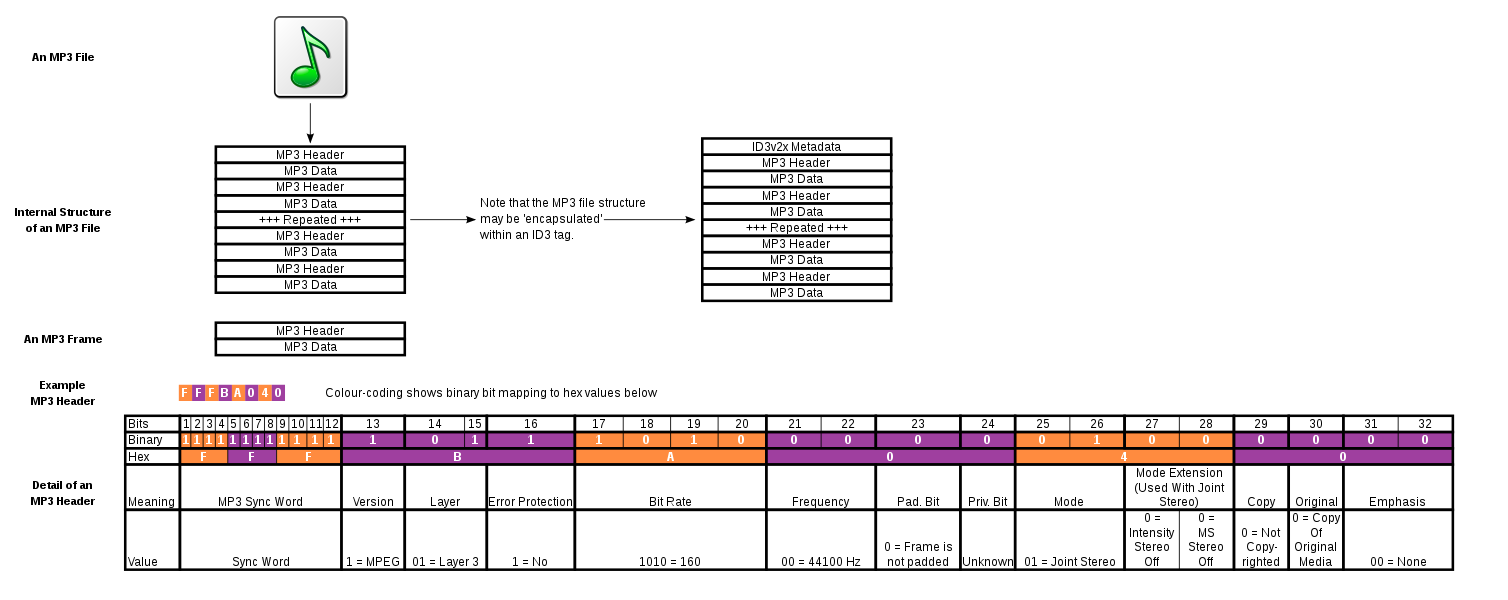
\includegraphics[width=\textwidth]{figs/mp3_file_structure.png}
         \caption{ساختار فایل MP3}
         \label{mp3_structure}
 \end{figure}

